\chapter{Wyniki badań i interpretacja modeli}
\label{chap:wyniki-interpretacja-modeli}

\providecommand{\ChapterFiveFigure}[3]{%
\begin{figure}[htbp]
\centering
\IfFileExists{#1}{%
    \includegraphics[width=0.92\textwidth]{#1}%
}{%
    \fbox{%
        \begin{minipage}[c][0.25\textheight][c]{0.86\textwidth}
        \centering
        \small Brak pliku graficznego w repozytorium:\\[4pt]
        {\scriptsize\texttt{\detokenize{#1}}}
        \end{minipage}%
    }%
}%
\caption{#2}
\label{#3}
\end{figure}%
}

\section{Ramy interpretacyjne rozdziału}
\label{sec:ramy-interpretacyjne-rozdzialu}

Ten rozdział zbiera wyniki po dwóch wcześniejszych etapach pracy: przygotowaniu danych i opisaniu metod. Punktem wyjścia jest 162 390 dopasowanych epizodów pobytu (przyjęcie--wynik) psów i kotów. Modele oceniano w porządku chronologicznym, a nie po losowym przemieszaniu rekordów: lata 2013--2021 posłużyły do uczenia, lata 2022--2023 do walidacji i ustawiania progów decyzyjnych, natomiast lata 2024--2025 do jednego, końcowego testu. Takie ustawienie jest bardziej wymagające, ale lepiej przypomina sytuację, w której model ma pracować na danych z przyszłości.

Wyniki trzeba czytać z podziałem na dwa osobne zadania. Klasyfikacja odpowiada na pytanie o prawdopodobieństwo adopcji. Regresja szacuje liczbę dni do \emph{dowolnego} dopasowanego wyniku pobytu, a więc nie jest prostą miarą ,,szybkości adopcji''. W tej zmiennej mieszczą się także inne zakończenia, między innymi eutanazja i powrót do właściciela. Dlatego atrybut \texttt{days\_to\_adoption} pełni tu tylko funkcję pomocniczą i opisową. Klasyfikatory oceniano za pomocą ROC-AUC, PR-AUC, Precision, Recall i F1-Score, a regresję przez MAE, RMSE i MedAE.

W dalszej części najpierw zestawiono jakość modeli, a następnie wrócono do hipotez badawczych. Osobne miejsce zajmuje interpretacja modeli, ponieważ same metryki nie wystarczają do oceny, czy wynik można rozsądnie wykorzystać w praktyce schroniskowej \cite{Lundberg2017}.

\section{Porównanie jakości modeli}
\label{sec:porownanie-jakosci-modeli}

Najpierw warto uporządkować całą ścieżkę analizy. Schemat pokazuje, jak od zbioru modelowego przechodzono do porównania algorytmów, wyboru modelu końcowego i interpretacji jego zachowania.

\begin{figure}[htbp]
\centering
\resizebox{0.98\textwidth}{!}{%
\begin{tikzpicture}[
    flowbox/.style={
        rectangle,
        rounded corners=3pt,
        draw=black,
        fill=LightGray,
        align=center,
        text width=3.4cm,
        minimum height=0.95cm,
        inner sep=5pt,
        font=\small
    },
    flowarrow/.style={-{Latex[length=2.4mm,width=1.8mm]}, thick}
]
\node[flowbox, text width=4.0cm] (A) at (0,0) {Zbiór modelowy AAC};
\node[flowbox, text width=5.0cm] (B) at (0,-1.45) {Podział chronologiczny\\trening -- walidacja -- test};
\node[flowbox] (C) at (-4.4,-3.15) {Modele bazowe};
\node[flowbox] (D) at (0,-3.15) {HistGradientBoosting};
\node[flowbox] (E) at (4.4,-3.15) {CatBoost};
\node[flowbox, text width=4.0cm] (F) at (0,-4.85) {Porównanie metryk};
\node[flowbox, text width=4.0cm] (G) at (0,-6.30) {Wybór modelu końcowego};
\node[flowbox, text width=3.9cm] (H) at (-2.7,-8.00) {Analiza progów\\i kalibracji};
\node[flowbox, text width=3.9cm] (I) at (2.7,-8.00) {Interpretacja globalna\\i lokalna};
\node[flowbox, text width=5.2cm] (J) at (0,-9.70) {Wnioski dla rozdziału wynikowego};

\foreach \from/\to in {A/B,B/C,B/D,B/E,C/F,D/F,E/F,F/G,G/H,G/I,H/J,I/J}{
    \draw[flowarrow] (\from) -- (\to);
}
\end{tikzpicture}%
}
\caption{Logika ewaluacji modeli klasyfikacyjnych i regresyjnych.}
\label{fig:logika-ewaluacji-modeli}
\end{figure}

Na zbiorze testowym z lat 2024--2025 nie wygrał jeden model ,,do wszystkiego''. W klasyfikacji adopcji najlepiej poradził sobie HistGradientBoosting, natomiast w regresji długości pobytu najniższy błąd uzyskał CatBoost.

Różnica między zadaniami jest dobrze widoczna w metrykach. Klasyfikacja, z ROC-AUC około 0,840, okazała się stabilniejsza niż przewidywanie czasu pobytu, gdzie MAE wyniosło około 18,5 dnia. Warto też zwrócić uwagę na gatunek: wyniki dla kotów są lepsze niż dla psów. Może to oznaczać, że ścieżki pobytu kotów są w badanym materiale bardziej powtarzalne albo mniej zależne od nietypowych przypadków.

Na wykresach łatwiej zobaczyć skalę tej przewagi niż w samej tabeli. Rysunek~\ref{fig:model-comparison-classification-roc-auc} pokazuje, że modele boostingowe wyraźnie odsuwają się od modelu bazowego, którym była Regresja Logistyczna.

\ChapterFiveFigure{../reports/figures/model_comparison_classification_roc_auc.png}{Zbiorcze porównanie zdolności dyskryminacyjnej badanych algorytmów na zbiorze łącznym oraz podzbiorach gatunkowych.}{fig:model-comparison-classification-roc-auc}

Dokładne wartości metryk na odłożonym zbiorze testowym zebrano w tabeli~\ref{tab:wyniki-najlepszych-modeli}.

\begin{table}[htbp]
\centering
\caption{Wyniki najlepszych modeli na zbiorze testowym (2024--2025)}
\label{tab:wyniki-najlepszych-modeli}
\scriptsize
\resizebox{\textwidth}{!}{%
\begin{tabular}{|l|l|l|l|l|l|l|l|l|l|}
\hline
\rowcolor{LightGray}
\textbf{Zadanie} & \textbf{Podzbiór danych} & \textbf{Najlepszy model} & \textbf{Główna miara (ROC-AUC / MAE)} & \textbf{PR-AUC} & \textbf{F1-Score} & \textbf{Precision} & \textbf{Recall} & \textbf{RMSE} & \textbf{MedAE} \\
\hline
Klasyfikacja & Zbiór łączny & HistGradientBoosting & \textbf{0,840} (ROC-AUC) & 0,884 & 0,818 & 0,835 & 0,801 & -- & -- \\
\hline
Klasyfikacja & Psy & HistGradientBoosting & \textbf{0,806} (ROC-AUC) & 0,857 & 0,799 & 0,817 & 0,781 & -- & -- \\
\hline
Klasyfikacja & Koty & HistGradientBoosting & \textbf{0,865} (ROC-AUC) & 0,899 & 0,842 & 0,846 & 0,839 & -- & -- \\
\hline
Regresja & Zbiór łączny & CatBoost & \textbf{18,55} (MAE dni) & -- & -- & -- & -- & 38,36 & 6,28 \\
\hline
Regresja & Psy & CatBoost & \textbf{21,56} (MAE dni) & -- & -- & -- & -- & 45,99 & 6,28 \\
\hline
Regresja & Koty & CatBoost & \textbf{15,79} (MAE dni) & -- & -- & -- & -- & 30,12 & 5,71 \\
\hline
\end{tabular}%
}
\end{table}

\begin{figure}[htbp]
\centering
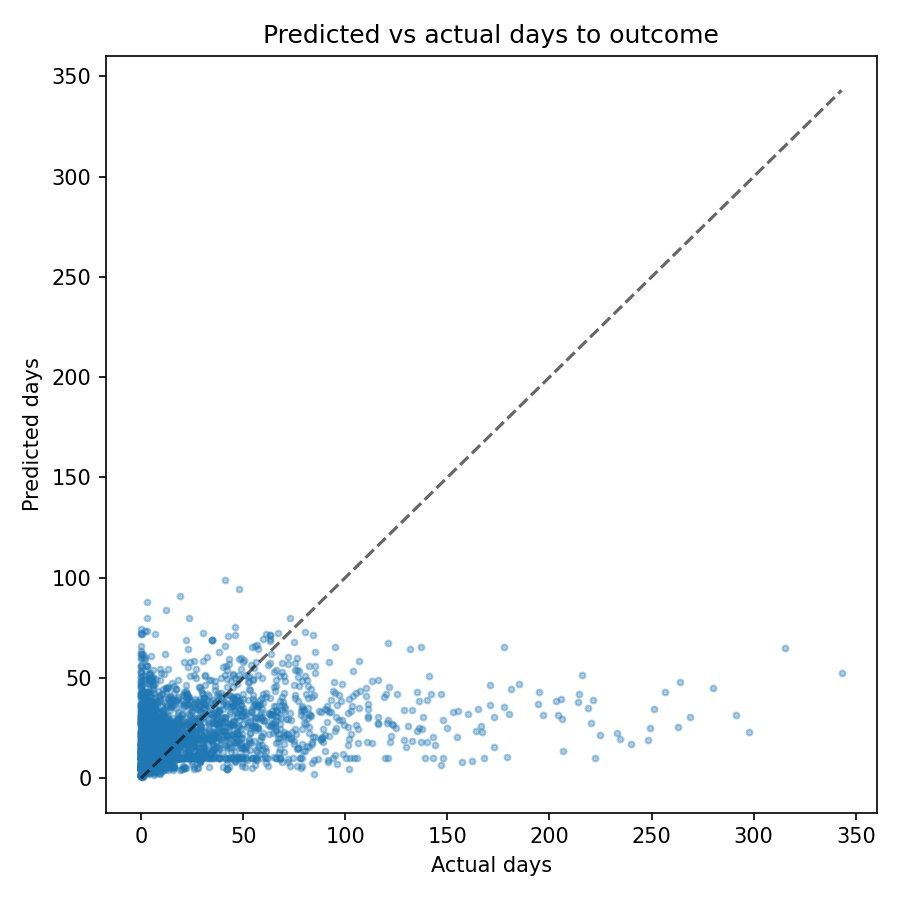
\includegraphics[width=0.88\textwidth]{../reports/figures/diagnostic_predicted_vs_actual.png}
\caption{Wartości rzeczywiste kontra przewidywane dla modelu regresyjnego (CatBoost). Widoczny jest systematyczny niedoszacunek dla długich pobytów (powyżej 60~dni).}
\label{fig:diagnostic-predicted-vs-actual}
\end{figure}

\begin{figure}[htbp]
\centering
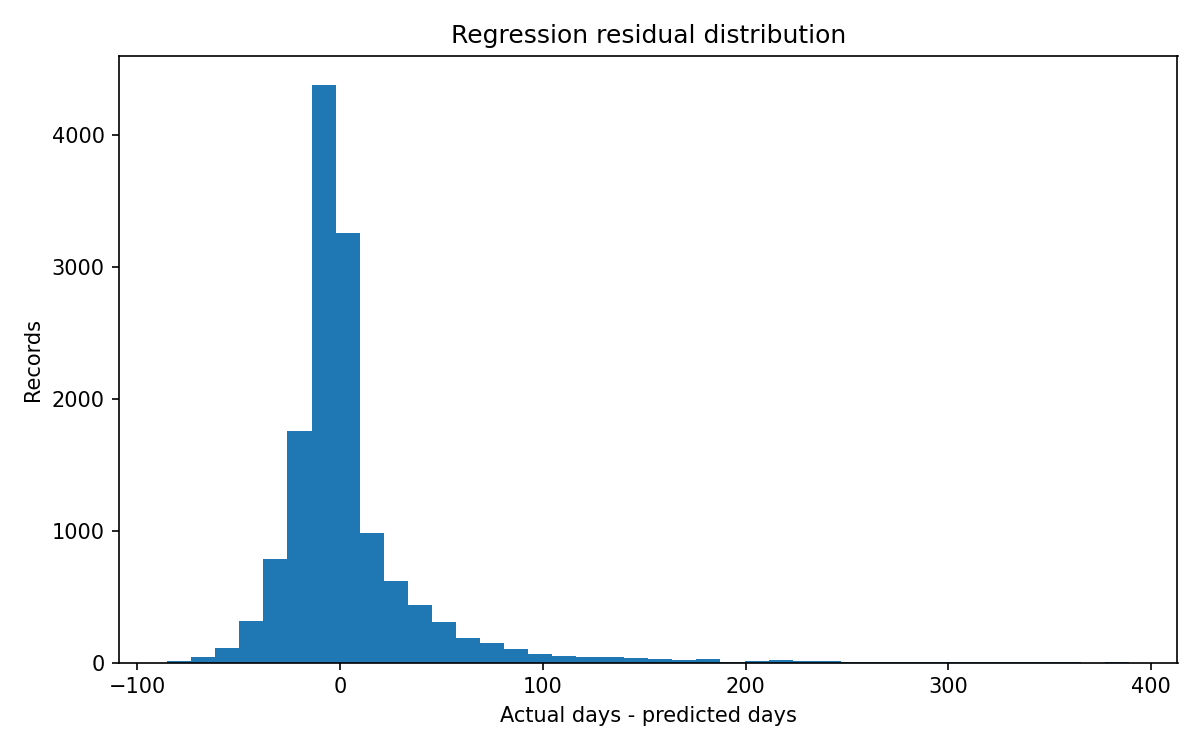
\includegraphics[width=0.88\textwidth]{../reports/figures/diagnostic_regression_residuals.png}
\caption{Rozkład reszt modelu regresyjnego. Silna asymetria prawostronna potwierdza koncentrację błędów na rzadkich przypadkach bardzo długich pobytów -- MAE wynosi 18{,}55~dnia, natomiast mediana błędu zaledwie 6{,}28~dnia.}
\label{fig:diagnostic-regression-residuals}
\end{figure}

Te liczby potwierdzają, że modele bazowe spełniły swoją rolę kontrolną. Naiwne przewidywanie mediany lub dominanty pozwalało sprawdzić, czy dane niosą jakikolwiek sygnał predykcyjny. Najwięcej informacji analitycznej dały jednak modele boostingowe, zgodnie z szerszymi wynikami badań nad danymi tabelarycznymi \cite{Chen2016,Prokhorenkova2018,Grinsztajn2022}. Regresja logistyczna pozostaje użyteczna jako prostszy punkt odniesienia, ale to modele nieliniowe lepiej wykorzystały strukturę danych tabelarycznych.

\ChapterFiveFigure{../reports/figures/diagnostic_roc_curve.png}{Szczegółowy przebieg krzywej ROC dla zwycięskiego klasyfikatora (HistGradientBoosting). Widoczne wyraźne wysklepienie nad linią losową (AUC = 0.50).}{fig:diagnostic-roc-curve}

Uzupełnieniem analizy skuteczności klasyfikatora jest krzywa Precision-Recall (PR) oraz macierz pomyłek, które dokładniej ilustrują rozkład błędów modelu, a w szczególności proporcje wyników fałszywie pozytywnych (FP) względem fałszywie negatywnych (FN). W kontekście schroniskowym minimalizowanie obu typów błędów ma inne konsekwencje praktyczne: błędne wskazanie na wysoką szansę adopcji (FP) może opóźnić konieczne interwencje wspomagające, a zbyt pesymistyczna prognoza (FN) prowadzić do marnowania zasobów na zwierzę, które poradziłoby sobie samo.

\ChapterFiveFigure{../reports/figures/diagnostic_precision_recall_curve.png}{Krzywa Precision-Recall dla najlepszego modelu klasyfikacyjnego. Pozwala lepiej ocenić jakość predykcji, zwłaszcza w sytuacji niezbalansowania klas.}{fig:diagnostic-pr-curve}

\ChapterFiveFigure{../reports/figures/final_confusion_matrix.png}{Macierz pomyłek dla modelu końcowego, pozwalająca szczegółowo prześledzić rozkład poprawnych i błędnych klasyfikacji.}{fig:final-confusion-matrix}

Osobno sprawdzono cechy kontekstowe, takie jak pogoda i wcześniejszy wolumen przyjęć. Ich dodanie nie przyniosło dużej, jednolitej poprawy we wszystkich rodzinach modeli. W klasyfikacji pojawił się niewielki zysk dla CatBoosta w zbiorze łącznym, ale nie przełożył się on na wyraźną poprawę dla psów. W praktyce oznacza to, że zewnętrzny kontekst środowiskowy w momencie przyjęcia należy traktować ostrożnie, raczej jako uzupełnienie niż główne źródło informacji.

\subsection{Porównanie modeli regresyjnych}

W zadaniu regresji szacującym liczbę dni do wyjścia ze schroniska, najlepsze wyniki uzyskał CatBoost. Do oceny tego zadania wykorzystano metryki opierające się na różnicy między predykcją a wartością rzeczywistą: średni błąd bezwzględny (MAE) oraz pierwiastek błędu średniokwadratowego (RMSE). Rysunki \ref{fig:model-comparison-regression-mae} i \ref{fig:model-comparison-regression-rmse} pokazują graficzne zestawienie błędów dla poszczególnych algorytmów. 

\ChapterFiveFigure{../reports/figures/model_comparison_regression_mae.png}{Porównanie badanych algorytmów pod kątem średniego błędu bezwzględnego (MAE) na zbiorze łącznym oraz podzbiorach gatunkowych.}{fig:model-comparison-regression-mae}

\ChapterFiveFigure{../reports/figures/model_comparison_regression_rmse.png}{Zestawienie błędu RMSE dla modeli regresyjnych. Wyższa waga większych odchyleń uwypukla przewagę CatBoosta nad innymi algorytmami.}{fig:model-comparison-regression-rmse}

Modele boostingowe, a zwłaszcza CatBoost, poradziły sobie z tym wyzwaniem zauważalnie lepiej od średniej czy mediany bazowej. Algorytm ten jest w stanie optymalnie wyłapać nieliniowe relacje w strukturze danych wejściowych, co ma kluczowe znaczenie przy zjawiskach z dużą liczbą wartości odstających.

\section{Weryfikacja hipotez badawczych}
\label{sec:weryfikacja-hipotez-badawczych}

Każda z pięciu hipotez weryfikowana jest poniżej zarówno na podstawie analizy opisowej, jak i wyników predykcyjnych modeli.

\textbf{Hipoteza H1 (Wpływ okoliczności przyjęcia w relacji do wyglądu)}

Wyniki wspierają hipotezę, że okoliczności przyjęcia mają większe znaczenie niż same cechy wyglądu. W analizie opisowej najwyższe wskaźniki adopcji pojawiają się przy zrzeczeniu właścicielskim (\texttt{Owner Surrender}) oraz kategorii \texttt{Abandoned}. Podobny obraz widać w modelu: analizy SHAP i ablacja Rodzin Cech wskazują silniejszy sygnał po stronie zmiennych opisujących typ i okoliczności przyjęcia niż po stronie koloru czy innych cech wyglądu. Nie jest to dowód przyczynowy. To raczej spójna asocjacja, którą model wykorzystuje przy predykcji; podobną potrzebę ostrożności przy interpretowaniu cech schroniskowych podkreślają wcześniejsze badania nad adopcją i długością pobytu \cite{Bradley2021,Cain2020}.

\ChapterFiveFigure{../reports/figures/h1_feature_family_importance.png}{Porównanie ważności rodzin cech dla wyniku klasyfikacji. Cechy okoliczności przyjęcia (Intake) dominują nad wyglądem.}{fig:h1-feature-family-importance}

\textbf{Hipoteza H3 (Wpływ wieku zwierzęcia)}

W przypadku wieku zależność jest czytelna i zgodna z intuicją oraz wcześniejszymi badaniami nad wynikami schroniskowymi \cite{Cain2020,Bradley2021}. Najmłodsze zwierzęta najczęściej kończyły pobyt adopcją: grupa \texttt{Baby} osiąga wskaźnik 59,7\%. Dla grupy \texttt{Young} jest to 47,5\%, dla zwierząt dorosłych 39,6\%, a dla seniorów 31,0\%. Wiek pojawia się też wysoko w globalnych wyjaśnieniach modelu, więc nie jest to wyłącznie efekt prostego zestawienia opisowego.

\ChapterFiveFigure{../reports/figures/h3_age_adoption_rate.png}{Spadek prawdopodobieństwa adopcji postępujący wraz z wiekiem zwierzęcia (w latach).}{fig:h3-age-adoption-rate}

\begin{figure}[htbp]
\centering
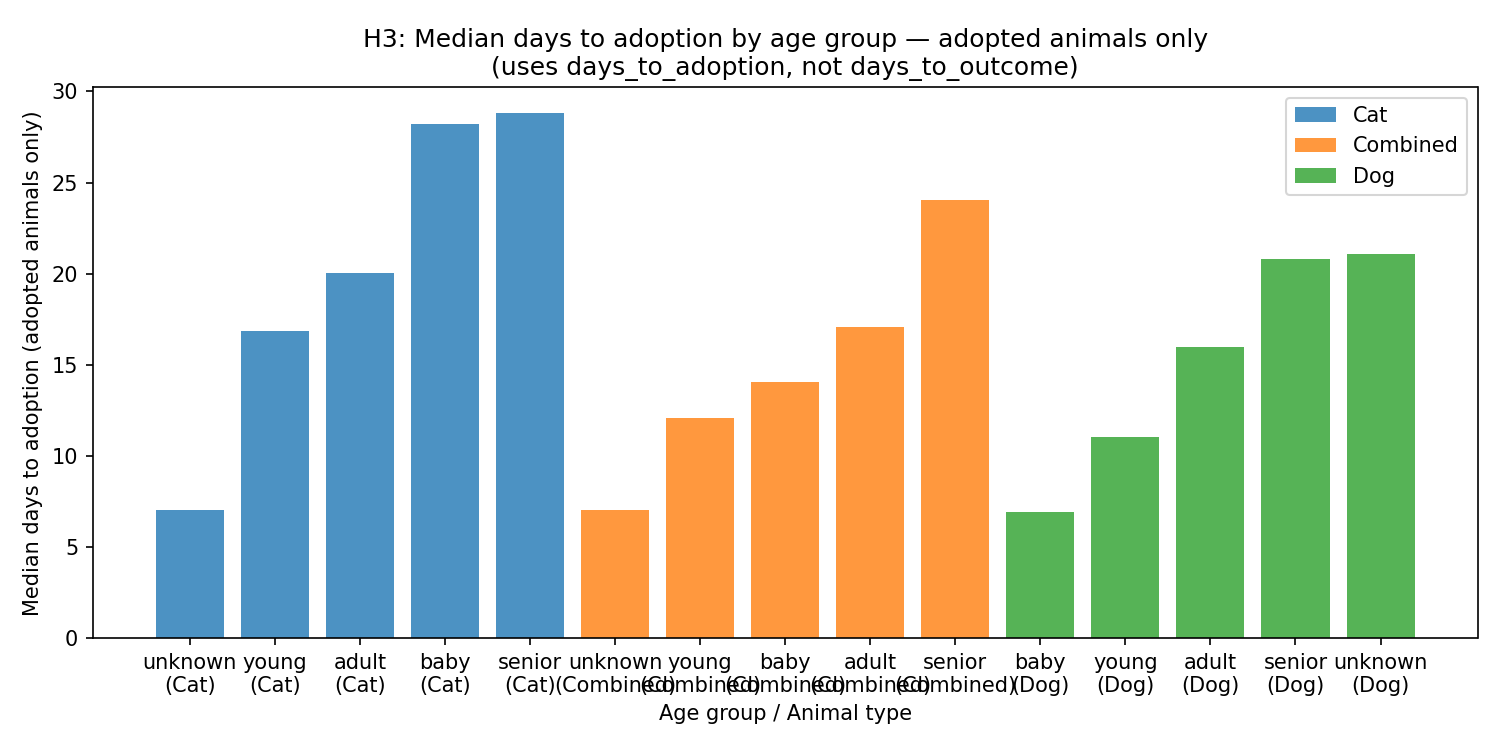
\includegraphics[width=0.88\textwidth]{../reports/figures/h3_adopted_only_median_days_to_adoption.png}
\caption{Mediana liczby dni do adopcji w podziale na grupy wiekowe (wyłącznie zwierzęta adoptowane). Niemowlęta opuszczają schronisko najszybciej.}
\label{fig:h3-adopted-only-median-days}
\end{figure}

\begin{figure}[htbp]
\centering
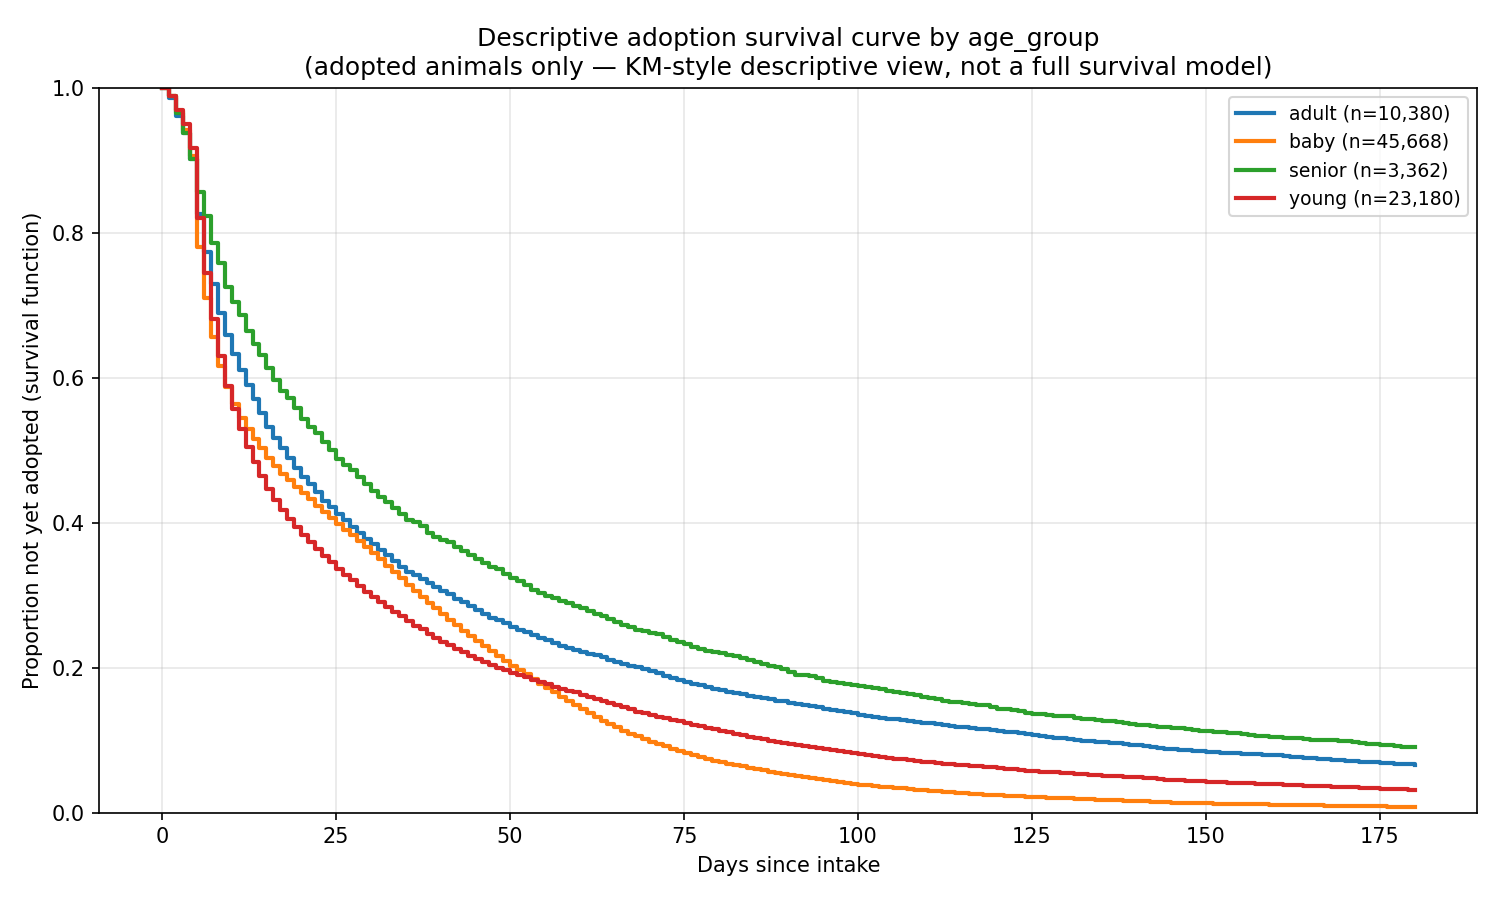
\includegraphics[width=0.88\textwidth]{../reports/figures/km_adoption_by_age_group.png}
\caption{Krzywe Kaplana-Meiera dla adopcji w podziale na grupy wiekowe~\cite{Kaplan1958}. Stromszy przebieg krzywej dla grupy \texttt{baby} potwierdza szybszy czas wyjścia ze schroniska.}
\label{fig:km-adoption-by-age-group-ch5}
\end{figure}

\textbf{Hipoteza H5 (Okres pandemii COVID-19)}

Okres COVID-19 nie daje się sprowadzić do prostej historii o większym popycie na adopcje. W danych opisowych widać wzrost odsetka adopcji: z 46,3\% przed pandemią do 61,5\% po pandemii. Jednocześnie mediana liczby dni do opuszczenia schroniska rośnie z 5,25 do 9,83 dnia. Ten pozorny paradoks sugeruje zmianę struktury przyjmowanych zwierząt albo zmianę pojemności operacyjnej ośrodka, co jest spójne z obserwacjami o zmianach praktyk schroniskowych i przepływów zwierząt w pierwszym okresie pandemii \cite{Hawes2022,Gunter2022}. Zmniejszenie ogólnej liczby przyjęć w trakcie samej pandemii również jest czytelnym sygnałem zachodzących przemian. Sama informacja o pandemii pomaga więc opisać okres, ale nie powinna być czytana jako samodzielne wyjaśnienie mechanizmu.

\ChapterFiveFigure{../reports/figures/h5_covid_adoption_rate.png}{Różnice we wskaźnikach adopcji przed, w trakcie oraz po pandemii COVID-19.}{fig:h5-covid-adoption-rate}

\ChapterFiveFigure{../reports/figures/h5_covid_intake_volume.png}{Wolumen przyjęć w zależności od okresu względem pandemii COVID-19.}{fig:h5-covid-intake-volume}

\textbf{Hipoteza H2 (Wpływ sezonowości)}

Sezonowość w danych wykazuje pewne różnice, jednak w ogólnym ujęciu ma ona charakter drugorzędny i pomocniczy. Zauważalne są wahania wskaźników w zależności od pór roku, co widoczne jest zarówno we wskaźnikach adopcji, jak i w medianie czasu pobytu. Efekt ten nie przeważa nad takimi zmiennymi jak okoliczności przyjęcia.

\ChapterFiveFigure{../reports/figures/h2_adoption_rate_by_season.png}{Wskaźniki adopcji w rozbiciu na pory roku. Wiosna i lato wykazują wyższe wskaźniki niż jesień i zima.}{fig:h2-adoption-rate-by-season}

\ChapterFiveFigure{../reports/figures/h2_median_los_by_season.png}{Mediana czasu pobytu w zależności od sezonu.}{fig:h2-median-los-by-season}

\textbf{Hipoteza H4 (Ciemne umaszczenie i Black Dog Syndrome)}

Hipoteza o ciemnym umaszczeniu, nawiązująca do tak zwanego \emph{Black Dog Syndrome}, dotyczy przypuszczalnie niższych szans na adopcję dla zwierząt o ciemnym kolorze sierści. Historycznie, zwierzęta ujęte w kategorii \texttt{is\_black\_or\_dark} faktycznie osiągały nieco niższe wskaźniki adopcji. Obecne zestawienia pokazują jednak ciekawe zjawisko polegające na nieznacznym odwróceniu tego efektu -- można zaobserwować delikatne przełamanie \emph{Black Dog Syndrome}, gdyż zwierzęta ciemne zaczynają lokalnie zyskiwać w statystykach adopcyjnych. Wciąż jednak taki wynik ilustruje jedynie asocjację w danych, a nie przyczyny decyzji ludzi; literatura opisująca zjawisko preferencji ze względu na wygląd ostrzega, że wpływ koloru i rasy bywa wysoce niejednoznaczny \cite{svoboda2015,Gunter2016,Cain2020}.

\ChapterFiveFigure{../reports/figures/h4_dark_color_adoption_rate.png}{Porównanie wskaźnika adopcji ze względu na umaszczenie zwierząt, wskazujące na lekkie odwrócenie trendu dla grupy o ciemnym umaszczeniu.}{fig:h4-dark-color-adoption-rate}

\ChapterFiveFigure{../reports/figures/h4_dark_color_median_los.png}{Różnice w medianie czasu pobytu dla zwierząt z jasnym i ciemnym umaszczeniem.}{fig:h4-dark-color-median-los}

\begin{table}[htbp]
\centering
\caption{Status hipotez badawczych w świetle wyników}
\label{tab:status-hipotez-badawczych}
\small
\begin{tabular}{|p{0.10\textwidth}|p{0.22\textwidth}|p{0.22\textwidth}|p{0.34\textwidth}|}
\hline
\rowcolor{LightGray}
\textbf{Hipoteza} & \textbf{Zakres} & \textbf{Status} & \textbf{Najważniejsza obserwacja} \\
\hline
H1 & Okoliczności przyjęcia vs wygląd & Wsparta opisowo i predykcyjnie & Cechy intake-related wykazują wyższą doniosłość (SHAP importance) niż atrybuty umaszczenia. \\
\hline
H2 & Sezonowość & Analiza opisowa & Różnice sezonowe istnieją, ale stanowią czynnik drugorzędny predykcyjnie. \\
\hline
H3 & Wiek & Wsparta opisowo i predykcyjnie & Wskaźnik adopcji maleje z 59,7\% (\texttt{baby}) do 31,0\% (\texttt{senior}). \\
\hline
H4 & Ciemne umaszczenie & Analiza opisowa & Historycznie niższa adopcyjność ulegająca lokalnemu odwróceniu (lekkie przełamanie efektu). \\
\hline
H5 & Okres COVID-19 & Wsparta opisowo & Wzrost adopcji (z 46\% do 61\%) przy jednoczesnym wzroście czasu pobytu (z 5 do 9 dni mediany). \\
\hline
\end{tabular}
\end{table}

\section{Interpretacja i wiarygodność modelu}
\label{sec:interpretacja-wiarygodnosc-modelu}

Interpretacja modelu nie jest tu dodatkiem estetycznym, lecz warunkiem sensownego użycia wyników. W środowisku weterynaryjnym i schroniskowym decyzje dotyczą konkretnych zwierząt, dlatego model typu ,,czarna skrzynka'' (ang. \emph{black-box}) łatwo może budzić nieufność personelu. Pracownik schroniska powinien wiedzieć, dlaczego szczeniak albo starszy pies został oznaczony jako przypadek podwyższonego ryzyka. Do tego wykorzystano metody \emph{Explainable AI} (XAI), przede wszystkim wartości SHAP \cite{Lundberg2017}. Globalne wykresy SHAP są zgodne z intuicją wynikającą z danych: starszy wiek obniża prawdopodobieństwo adopcji, a młody wiek działa w przeciwnym kierunku. Taka zgodność nie rozwiązuje wszystkich problemów interpretacyjnych, ale ułatwia rozmowę o modelu z osobami, które miałyby z niego korzystać.

\ChapterFiveFigure{../reports/figures/shap_summary_classification.png}{Zbiorczy wykres SHAP (Summary Plot) dla zadania klasyfikacji, obrazujący wpływ poszczególnych wartości cech na przewidywane prawdopodobieństwo adopcji.}{fig:shap-summary-classification}

\ChapterFiveFigure{../reports/figures/shap_feature_families_classification.png}{Zestawienie średnich wartości SHAP według rodzin cech dla klasyfikatora adopcji. Rodzina \texttt{name\_identity} uzyskała najwyższy sumaryczny wkład predykcyjny ($\approx$~0{,}55), wyprzedzając cechy wiekowe ($\approx$~0{,}48) oraz rasowo-wyglądowe ($\approx$~0{,}26).}{fig:shap-feature-families-classification}

Wynik ten wymaga komentarza. Zmienna \texttt{has\_name} (czy zwierzę miało imię w chwili przyjęcia) nie oznacza, że samo nadanie imienia zwiększa szansę adopcji -- jest to asocjacja agregująca wiele kontekstów właścicielskich. Efekt predykcyjny jest jednak na tyle silny, że dominuje nad cechami wyglądu, wiekiem i rasą~\cite{Lundberg2020}.

\ChapterFiveFigure{../reports/figures/shap_summary_regression.png}{Zbiorczy wykres SHAP dla regresji czasu pobytu, pokazujący w jaki sposób dane parametry wydłużają lub skracają prognozowany wynik.}{fig:shap-summary-regression}

Trzeba przy tym uczciwie zaznaczyć jedną decyzję metodologiczną. Najlepszym klasyfikatorem na teście był HistGradientBoosting, ale pełne wygenerowanie wykresów SHAP jest, ze względów narzędziowych i dostępności \emph{TreeExplainer}, wygodniejsze dla CatBoosta. Z tego powodu część interpretacji opiera się na modelach wspomagających. Służą one do pokazania kierunków zależności, a nie do zastępowania właściwej oceny modelu końcowego.

Drugim filarem użyteczności jest kalibracja. Samo wysokie ROC-AUC mówi, że model dobrze porządkuje przypadki, ale nie gwarantuje jeszcze, że podawane prawdopodobieństwa są dobrze wyskalowane \cite{Fawcett2006,Brier1950}. To szczególnie ważne na krańcach rozkładu predykcji, gdzie błędna pewność modelu może być bardziej kłopotliwa niż pojedyncza pomyłka klasyfikacyjna.

\ChapterFiveFigure{../reports/figures/diagnostic_calibration_curve.png}{Krzywa kalibracyjna (Calibration Curve) pokazująca, w jakim stopniu przewidywane przez model prawdopodobieństwo adopcji odpowiada rzeczywistej częstotliwości (Perfectly calibrated).}{fig:diagnostic-calibration-curve}

Oszacowania sprawdzono więc pod kątem luki kalibracyjnej (Brier Score) oraz progów decyzyjnych (\texttt{threshold}). Progi dobrano na niezależnym zbiorze walidacyjnym z lat 2022--2023, a potem przeniesiono bez zmian na test z lat 2024--2025. Dla małych podgrup, poniżej 100 obserwacji w zbiorze testowym, wyniki należy czytać szczególnie ostrożnie.

\subsection{Analiza błędów i wiarygodność modelu}

Istotnym aspektem sprawdzania jakości prognozy na wdrożeniu jest identyfikacja tych segmentów, w których algorytmy radzą sobie wyraźnie gorzej. Wykonano tzw. \emph{error analysis} przez wyizolowanie przekrojów (ang. \emph{error slices}) najczęściej prowadzących do pomyłki modelu. Dla klasyfikatora pozwala to wskazać konkretne podgrupy zwierząt wywołujące największy odsetek nietrafionych prognoz, podczas gdy w regresji rzuca światło na przypadki z nadzwyczaj wysokim błędem MAE.

\ChapterFiveFigure{../reports/figures/diagnostic_classification_error_slices.png}{Wizualizacja przekrojów błędu dla modelu klasyfikacyjnego. Ukazuje wycinki zbioru, w których skuteczność modelu jest najniższa.}{fig:diagnostic-classification-error-slices}

\ChapterFiveFigure{../reports/figures/diagnostic_regression_error_slices.png}{Analiza segmentacyjna błędów regresji. Rozbicie przypadków według wielkości MAE dla różnych profili zwierząt.}{fig:diagnostic-regression-error-slices}

Najostrożniej trzeba interpretować regresję czasu pobytu. Proces opuszczania schroniska jest częściowo losowy i zależy od czynników, których nie ma w tabeli danych. Model nie jest więc ,,wyrocznią'' wskazującą dokładny dzień wyjścia psa czy kota ze schroniska. Lepiej traktować go jako filtr ryzyka i narzędzie do porządkowania uwagi personelu. Z takiego założenia wynika późniejsza architektura Dashboardu oraz środowiska MLOps opisana w kolejnym rozdziale.